\section{What is the LSDF-Portal}

\begin{frame}[c]{TODOS}
    \todo{Write mail to Sundermann: Deployment (version updates, installs, constrain to django3} \\
    \todo{Write Changelog} \\
    \todo{Implement last features: publications sortable, command with mail on end\_date near} \\
\end{frame}


\subsection{Overview}
\begin{frame}[c]{What is the Large Scale Data Facility?}
    \large
    \begin{itemize}[<+(1)->]
        \item Cloud-based storage for scientific research
        \item About 18 PetaByte (1PB = 1000 TB)
        \item All commonly used Protocols
        \item Direct Integration with e.g. HoReKa HPC-systems
        \item Primarily for KIT, but also worldwide partners and Baden-Württemberg in general
        \item LSDF-Portal: {\em administration} of storage projects
    \end{itemize}
\end{frame}


\begin{frame}[c,fragile]{What is the LSDF-Portal?}
    \large
    \begin{itemize}[<+(1)->]
        \item LSDF-Portal: {\em administration} of storage projects
            \begin{itemize}[<+(1)->]
                \item Based on Python/Django (more on that later)
            \end{itemize}
        \item Research groups can request storage for timeframes
            \begin{itemize}[<+(1)->]
                \item And request extensions, should that not suffice
            \end{itemize}
        \item Internally available at \url{https://lsdf.kit.edu}
        \item My test instance available at \url{https://lsdf.fkarg.de}
        \item Play around with \verb!user:test! or \verb!admin4:lsdf! (both admin)
    \end{itemize}
\end{frame}

\begin{frame}[c]{Project Lifecycle}
    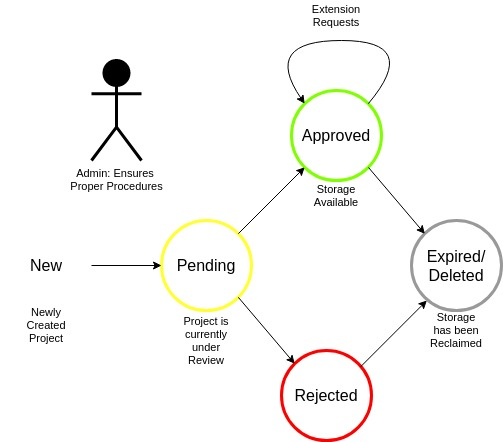
\includegraphics[height=0.9\textheight]{lsdf_states}
\end{frame}



\addtocounter{framenumber}{1}
\begin{frame}[standout]
    \Huge
    Live Demo!
\end{frame}

% \begin{frame}[c]
%     \todo{tell story: maths requesting storage for digitalization?}
% \end{frame}
\subsection{Project Creation}

\begin{frame}[c]{First Login}
                           % trim=left bottom right top, clip
    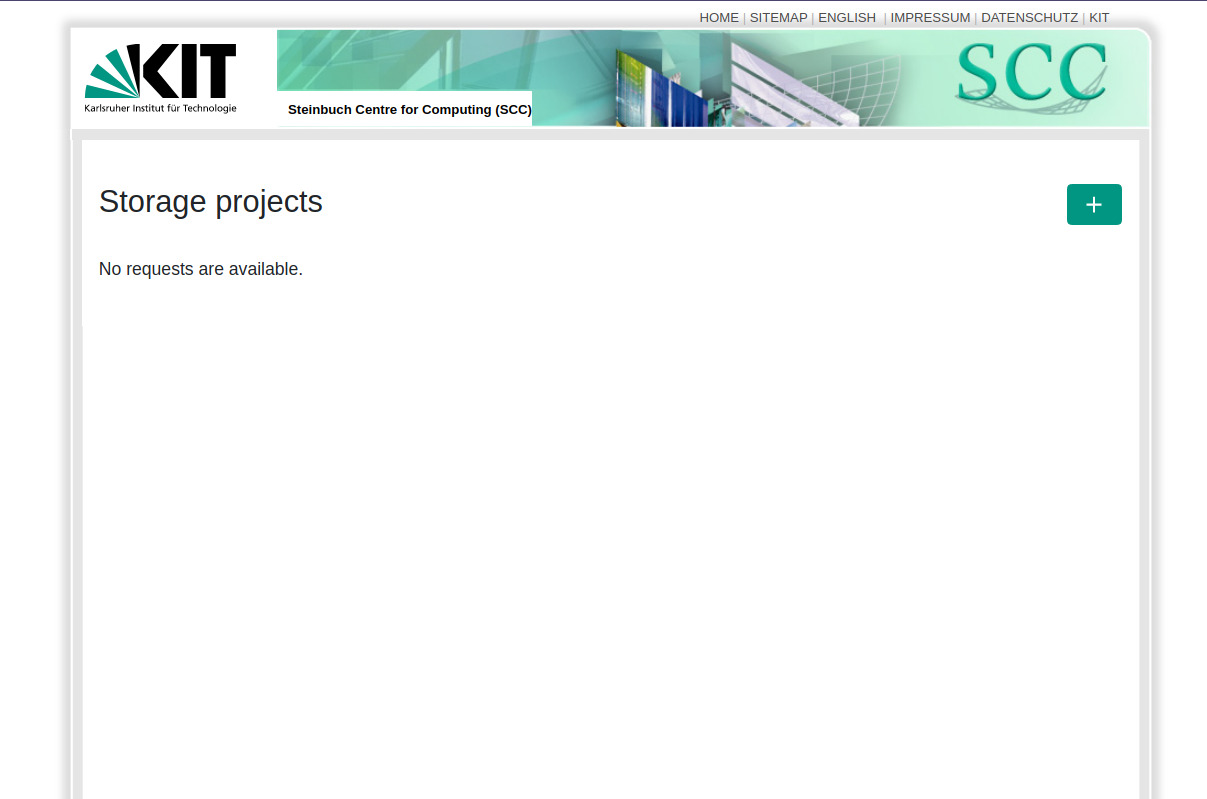
\includegraphics[width=\textwidth,trim=0 0 0 3,clip]{Selection_006}
\end{frame}

\begin{frame}[c]{Project Creation}
                           % trim=left bottom right top, clip
    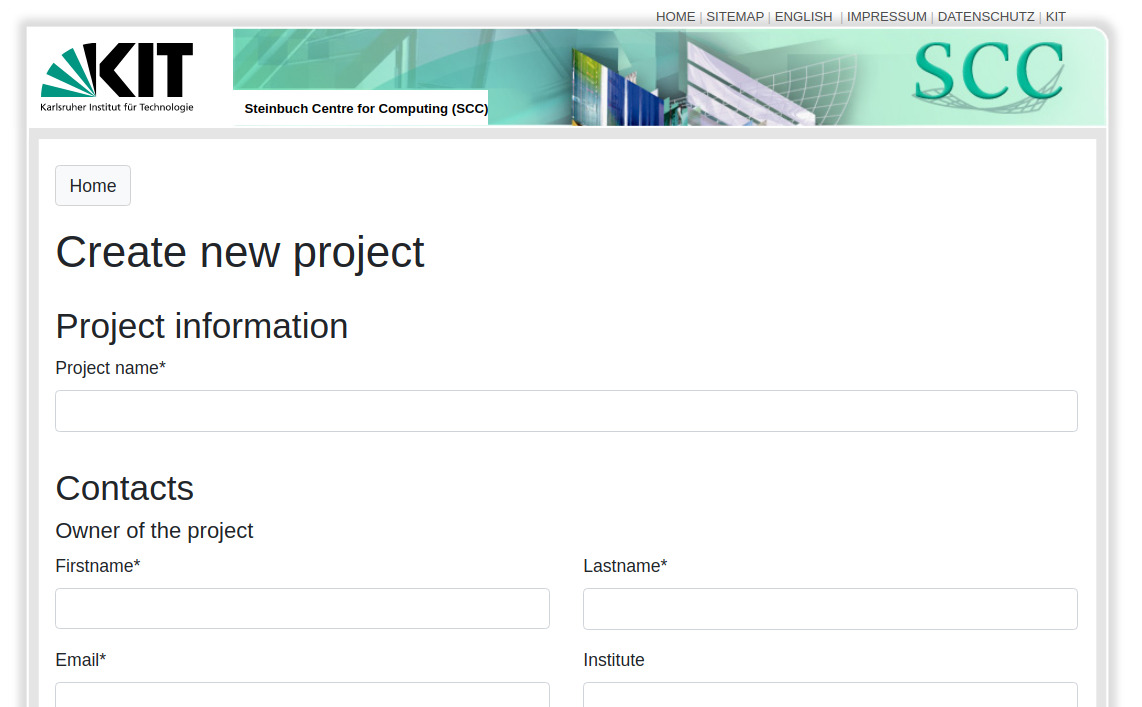
\includegraphics[width=\textwidth,trim=0 0 0 3,clip]{Selection_007}
\end{frame}

\begin{frame}[c]{Project Creation: Add Contacts}
                           % trim=left bottom right top, clip
    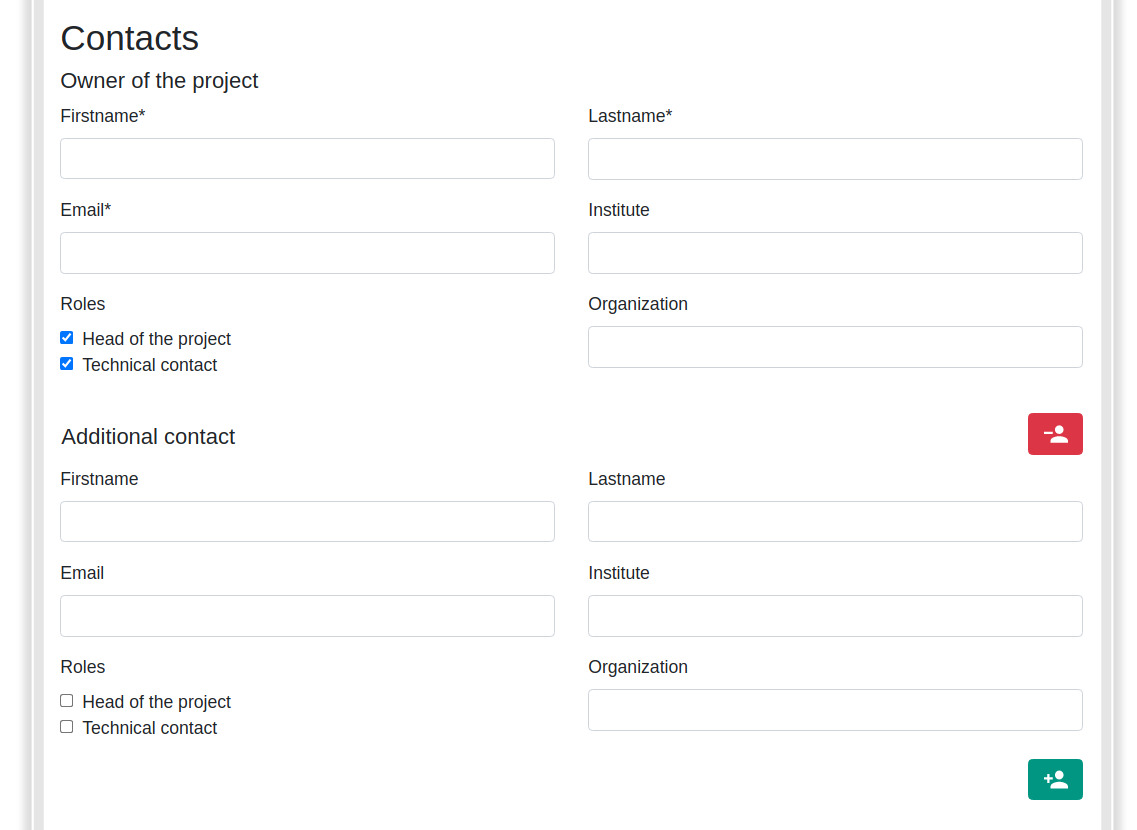
\includegraphics[width=\textwidth,trim=0 0 0 3,clip]{Selection_008}
\end{frame}

\begin{frame}[c]{Available Fields}
                           % trim=left bottom right top, clip
    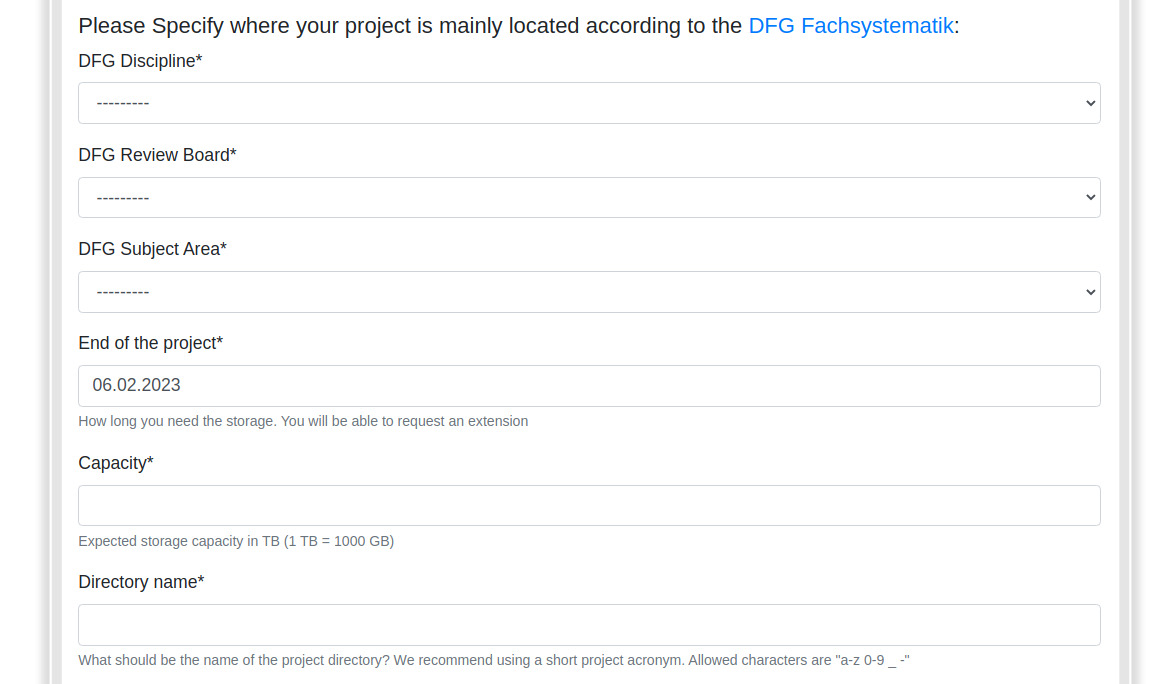
\includegraphics[width=\textwidth,trim=0 0 0 3,clip]{Selection_010}
\end{frame}

\begin{frame}[c]{Fields filled out}
                           % trim=left bottom right top, clip
    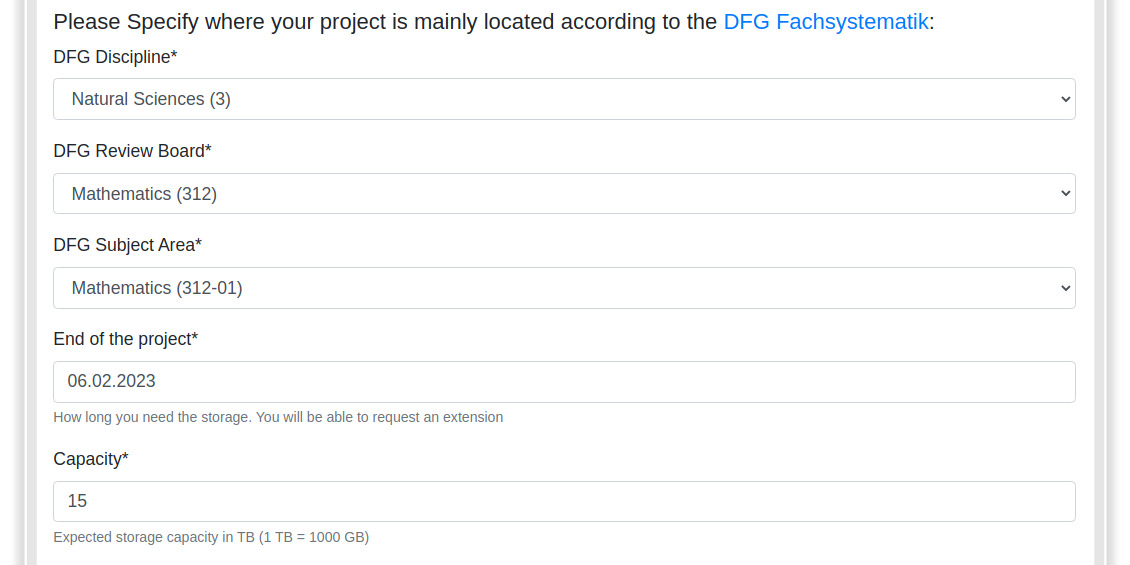
\includegraphics[width=\textwidth,trim=0 0 0 3,clip]{Selection_011}
\end{frame}

\begin{frame}[c]{Submit Proposal}
                           % trim=left bottom right top, clip
    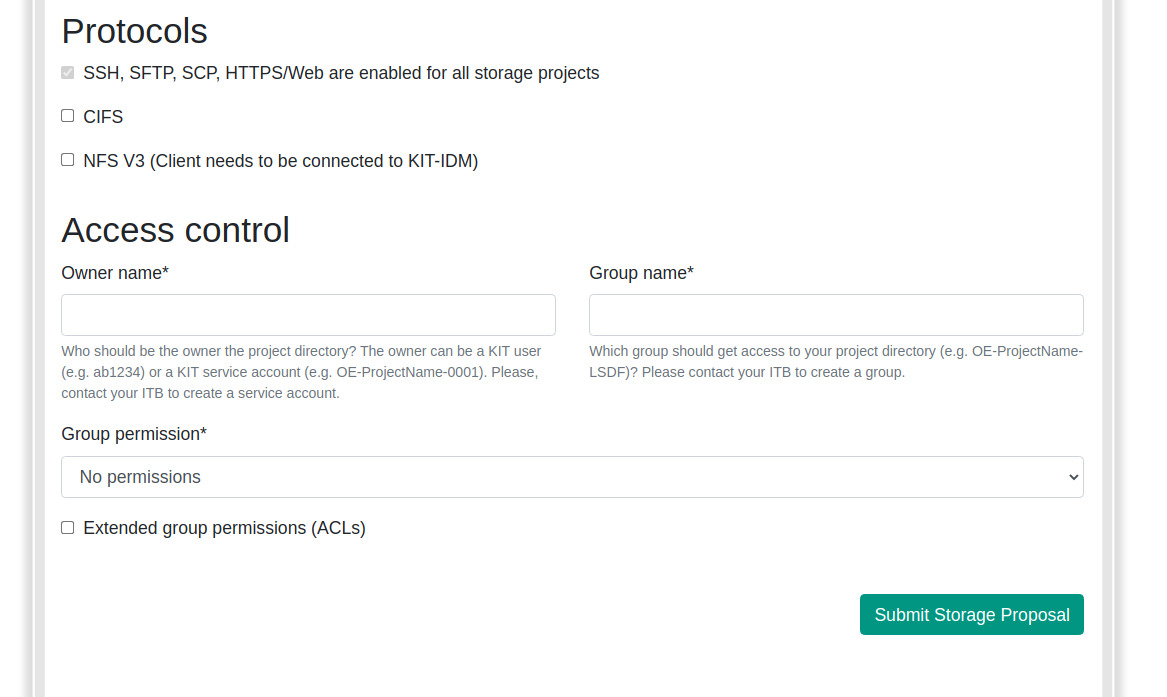
\includegraphics[width=\textwidth,trim=0 0 0 3,clip]{Selection_009}
\end{frame}

\begin{frame}[c]{Succesful Submission}
                           % trim=left bottom right top, clip
    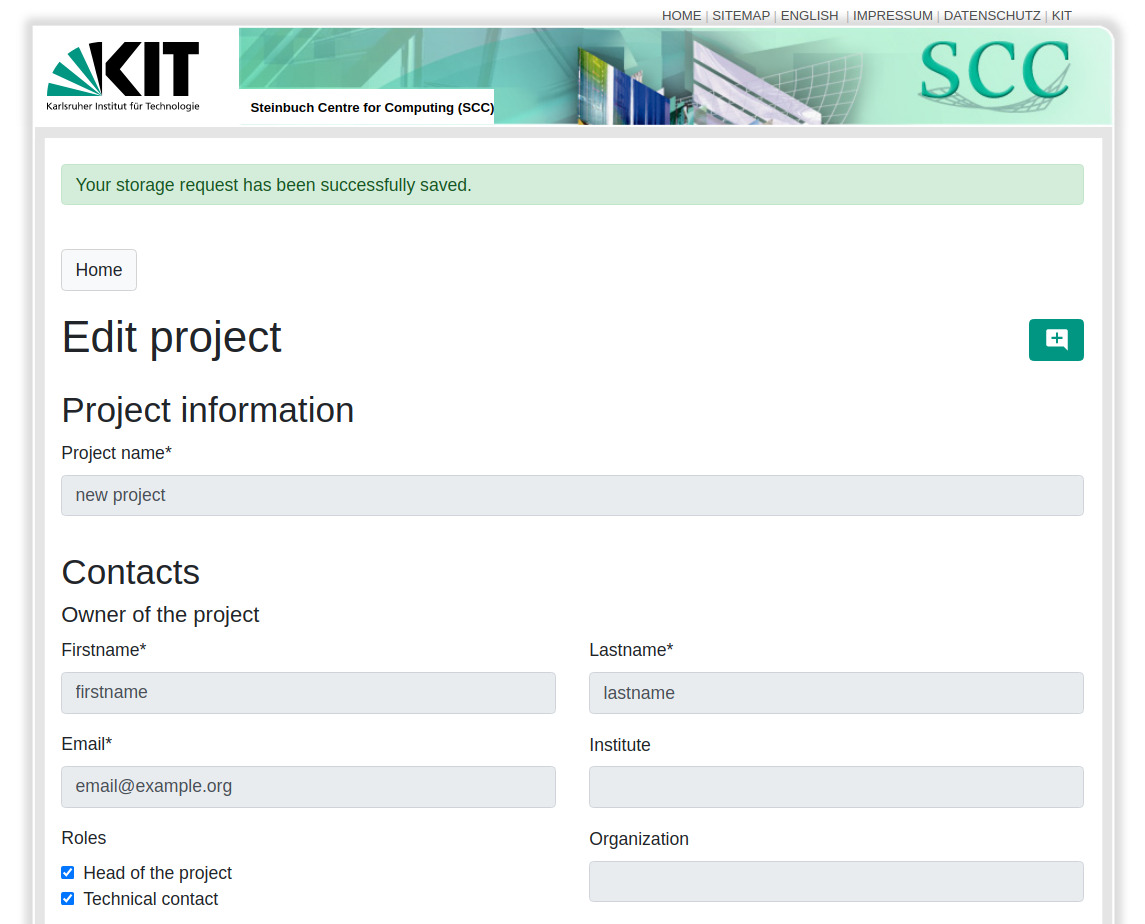
\includegraphics[width=\textwidth,trim=0 0 0 3,clip]{Selection_012}
\end{frame}

\begin{frame}[c]{Project in List}
                           % trim=left bottom right top, clip
    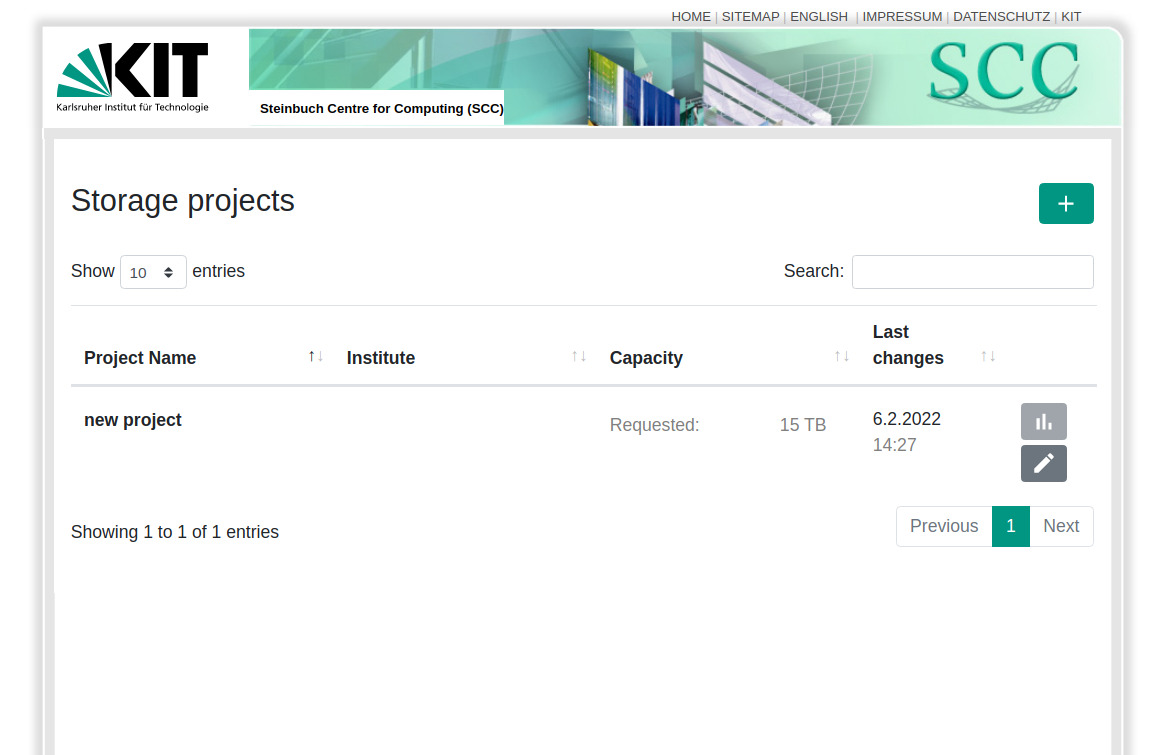
\includegraphics[width=\textwidth,trim=0 0 0 3,clip]{Selection_013}
\end{frame}

\subsection{Project Approval}
\pic{Project Pending}{14}
\pic{State Change Message}{15}
\pic{Project Approved}{17}
\pic{State Change Message}{16}

\subsection{Requesting More Storage}
\pic{Extension Requests: The Project Needs to be Approved}{18}
% \pic{Timeframe Extension Request View}{19}
\pic{lsdf.kit.edu/extension/timeframe/9/create/}{19}
\pic{Capacity Extension Request View}{20}
\pic{Filled out Capacity Extension}{21}
\pic{Extension System Message}{22}

\begin{frame}[c]{Projects Admin View}
                           % trim=left bottom right top, clip
    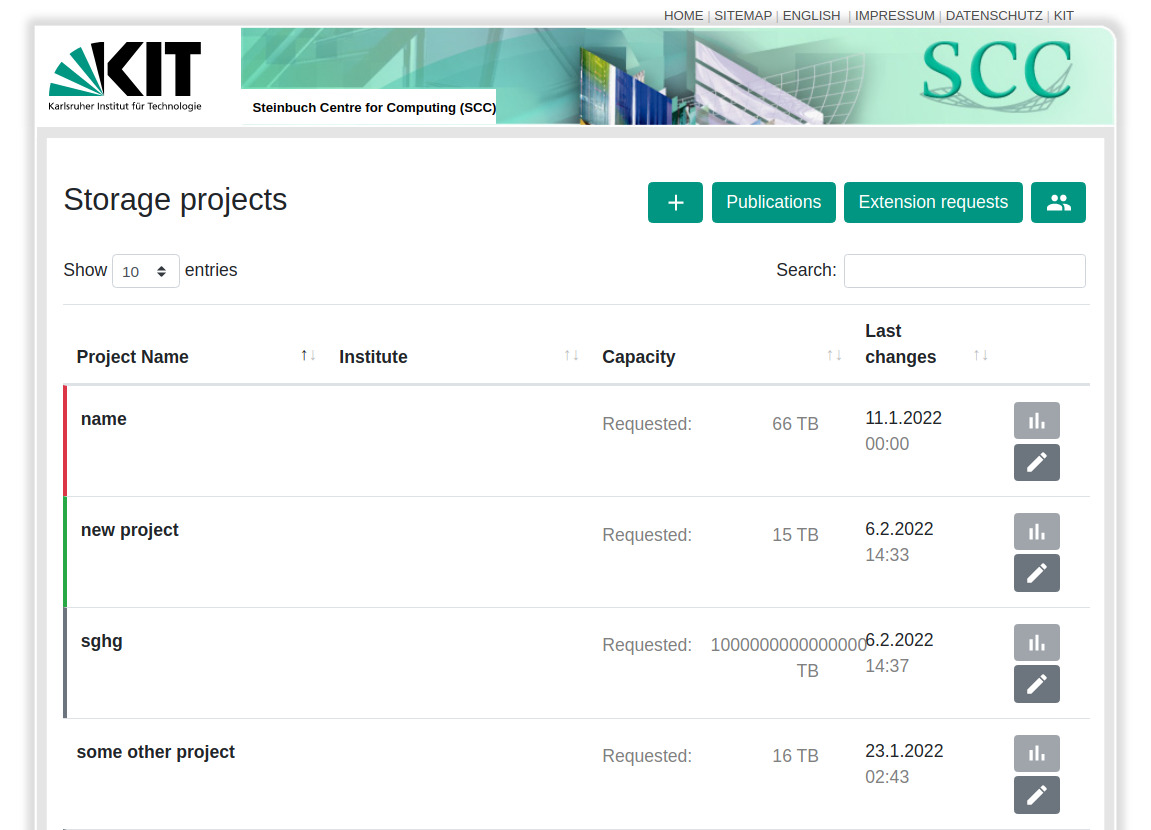
\includegraphics[width=\textwidth,trim=0 0 0 150,clip]{Selection_023}
\end{frame}

% 24 and 25 don't exist
\pic{Extension Request Overview}{26}
\pic{Approving Request}{27}
\pic{System Message showing Extension Approval}{28}
\pic{Increased Capacity from User View}{29}

\begin{frame}[c]{Storage Use Histogram}
    \todo{Screenshot: Histogram of storage usage. } \\
\end{frame}
